\documentclass[12pt,a4paper,final,twoside]{article}
\usepackage[utf8x]{inputenc}
\usepackage{ucs}
\usepackage{amsmath}
\usepackage[pdftex]{graphicx} 
\usepackage{amsfonts}
\usepackage{amssymb}
\usepackage{verbatim}
\usepackage[in]{fullpage}
\usepackage[bookmarks=true,colorlinks=true,linkcolor=black]{hyperref}
\usepackage[all]{hypcap}
\usepackage[small,bf]{caption}
\newcommand{\unit}[1]{\ensuremath{\, \mathrm{#1}}}
\graphicspath{{./img/}}
\begin{document}
\title{Technical Note: XMP16 many-core research board}
\author{Steve Kerrison}
\maketitle

This technical note is intended as a brief description of the University of Bristol \& XMOS ``XMP16'' many-core research boards, how to assemble them, how to write programs for them and how to run them. The boards and supporting tools are a work in progress. It is the responsibility of anyone who extends the tools to update this note accordingly, or produce a new, more in-depth set of documentation.

\section{XMP16 research board}

The XMP16 research boards were created by Dr. Simon Hollis and Jake Longo Galea in cooperation with XMOS.

\begin{figure}[htbp]
\centering
\setlength\fboxsep{0pt}
\setlength\fboxrule{1pt}
\fbox{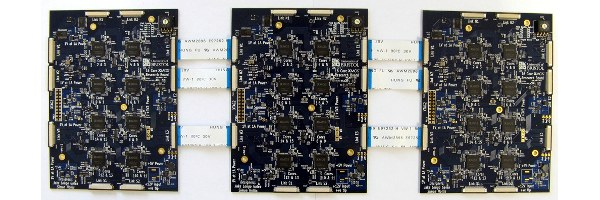
\includegraphics[scale=0.75,clip=true,trim=1.5cm 0 1.5cm 0]{xmp16x3.jpg}}
\caption{Three XMP16 boards in a horizontal configuration}
\end{figure}

The boards contain eight XMOS XS1-L2 dual-core chips, capable of operating at 500MHz, delivering up to eight threads per core at up to 500MIPS. These boards can be connected together to form arrays of XMP16s. The XS1 cores can communicate both on and off-board using XMOS XLinks. A JTAG chain is also formed across all interconnected boards, sharing the same ribbon cables as the XLinks.

\subsection{Key information}

Here we define some key elements of the operating characteristics of the boards.

\begin{tabular}{|c|c|p{2.5in}|}
\hline 
\textbf{Feature} & \textbf{Desc.} & \textbf{Detail} \\ 
\hline 
Core freq. & 500MHz & Configurable at both compile and run time \\ 
\hline 
Ref freq. & 100MHz & Keep at 100MHz to ensure consistent timing behaviour \\ 
\hline 
Link delays & "1,0" & As described in XN file, config register = 0xc0000800 \\ 
\hline 
Power supply & 12V @ ~2A & Power dissipation is workload \& freq. dependant. \\ 
\hline
JTAG & Via XTAG2 connector & Key should face into the board. \\
\hline 
\end{tabular}

\section{Physical configuration}

\subsection{Single board}

Single boards are very easy to operate. Supply them with 12V, configure the switch on the top-right of the board to value $7$, connect an XMOS XTAG2 programmer and use!

\begin{figure}[htbp]
\centering
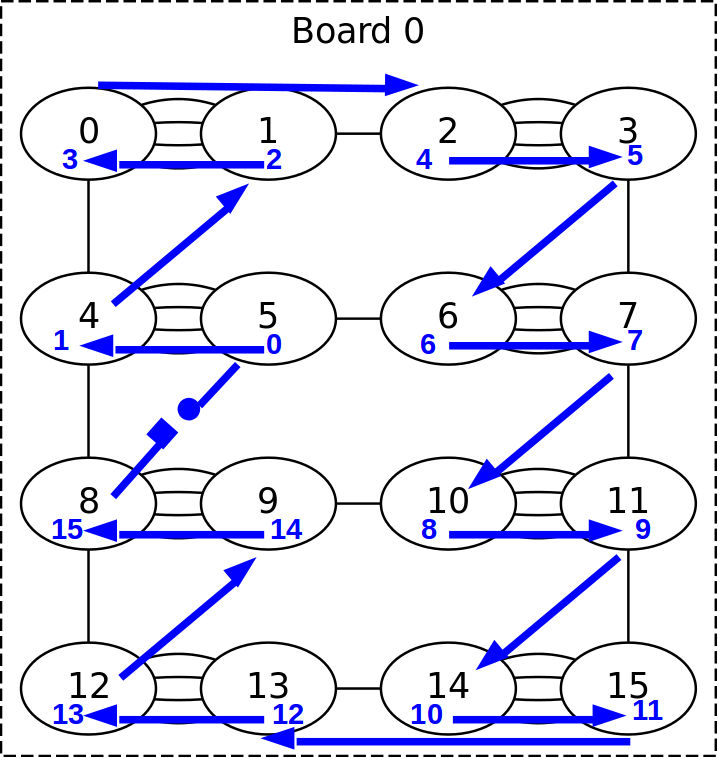
\includegraphics[scale=0.5]{jtag-single.png}
\caption{JTAG chain (blue) overlayed onto network node IDs of a single board. Note how the JTAG IDs do not correspond to the node IDs.}
\end{figure}

\subsection{Multiple boards}

To run multiple boards there are a few more steps:

\begin{enumerate}
\item Connect ribbon cables
\item Configure JTAG routing
\item Connect programmer to correct location
\end{enumerate}

\begin{figure}[htb]
\centering
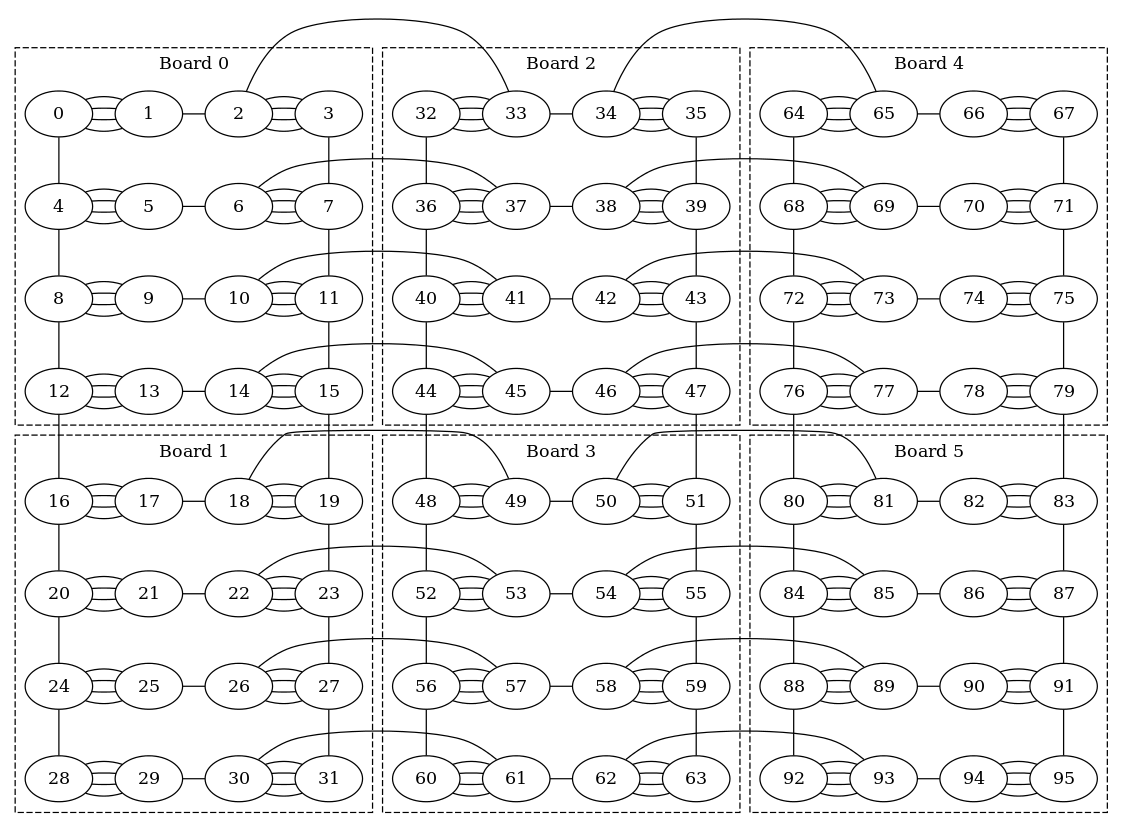
\includegraphics[scale=0.5]{xmp16-3x2-fixed.png}
\caption{Network topology of six boards arranged into two rows. The node IDs are the same as addressed by the XMOS channel layer and the \texttt{stdcore[n]} identification in XC.}
\end{figure}

\subsubsection{Ribbon cables}

Each board has 10 ribbon connectors. For a board to connect to another board in any direction, all ribbons on that edge must be connected to its neighbour.

Although the boards could conceivably be arranged into many configurations, the tools only support rectangular structures at this time. A board should always be connected to adjacent boards because the tools assume this.

\subsubsection{JTAG routing}

To allow for a JTAG chain to be formed in any board layout, the JTAG signals can be sent out over ribbon cables, or looped back in the case where there is no board connected in that direction. This is performed manually by a switch that is located at the top-right of the board which controls a number of multiplexers.

The control scheme is relatively simple. Each board edge, starting with north and moving clockwise, is represented in a 4-bit value by bits 0, 1, 2 and 3 respectively. If the bit is set, then the mux will loopback the signal. If not, it will go out over a ribbon connector on that edge.

Setting the switch to 7 (0b0111 - bits 0,1,2 are set, 3 is unset) configures the north, east and south edges in loopback, leaving the west open. This is the configuration required for a single board because the XTAG2 header occupies the same connections as the westbound connectivity and so the western edge must not be looped-back (doing so would create a cycle in the JTAG chain).

If we add a board to the south of our current board, then our current board needs bit 2 unset, giving us a switch value of 3 (0b0011). Assuming the new board is not connected to anything else, then its configuration would be 0xe (0b1110) so that only the north connection was open.

With this strategy any arrangement of boards can form a JTAG chain with a few provisions. Firstly, the XTAG2 connector can only ever be attached to the top-leftmost board. Secondly, the tools assume that the JTAG chain extends eastwards as far as it can, loops back towards the westmost board, then travels south one step before extending eastwards again.

It is important to note that node IDs, as viewed by programs and the routing tables, do not correspond to the position of cores in the JTAG chain. The tools, however, are capable of mapping between these.

\begin{figure}[htbp]
\centering
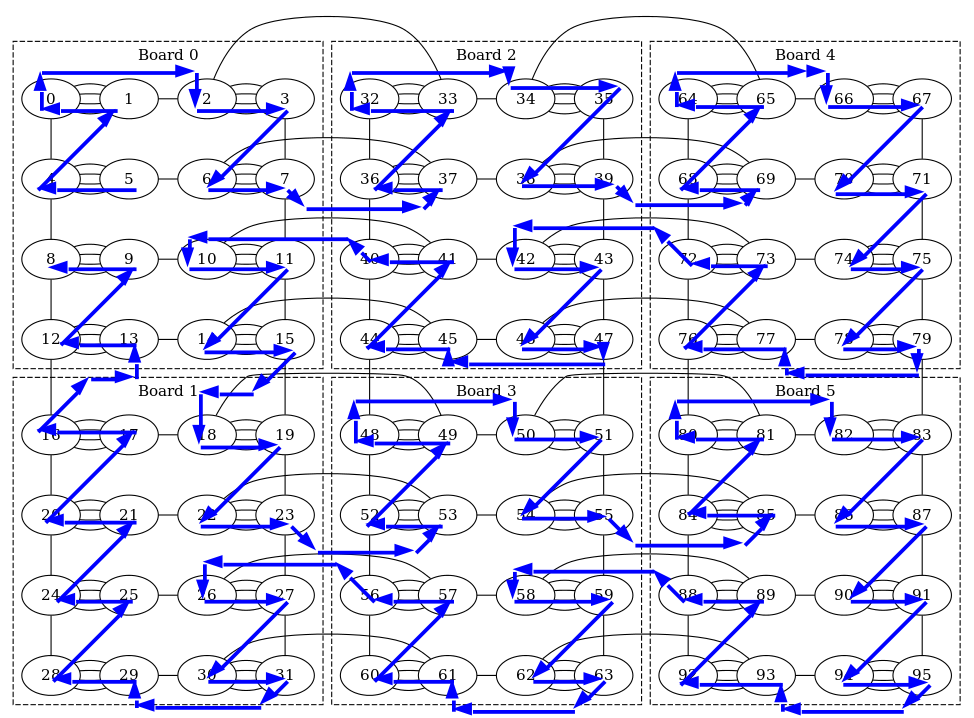
\includegraphics[scale=0.6]{jtag-3x2.png}
\caption{Crude depiction of JTAG chain on a multi-board array}
\end{figure}



\subsubsection{Connecting the programmer}

The XTAG2 programmer should always be attached to the top-leftmost board. Pin 1 is the bottom-rightmost pin on the header when viewing the board correctly oriented. The key on an XTAG2 connector should face inwards towards the centre of the XMP16. The westboard edge of this board should be set to open on the JTAG switch as described in the previous section.

\section{Software}

An array of XMP16 boards can be programmed using C, XMOS assembly and XMOS XC. In order to support large processor arrays, some wrappers are placed around the standard XMOS toolchain. These result in some deviations from what is traditionally possible in XMOS XC, but measures have been taken to reduce the impact of this.

\subsection{Required tools}

The following tools are required to program for an array of XMP16s:

\begin{itemize}
\item XMOS Development Suite (only version 11.11 is tested)
\item \texttt{scmake.py} - A parallel builder for per-core binaries
\item \texttt{xesection} - A tool to extract the program code from single-core XE files
\item \texttt{xebuilder.py} - A tool to assemble a many-core XE file from extracted sections.
\item \texttt{xmp16-routegen.py} - A script to generate routing tables and JTAG mappings for any given XMP16 array.
\item \texttt{xmp16-mcsc.py} - The multi-core to single-core compiler wrapper, providing reasonable compatibility with existing XMOS multi-core programming paradigms.
\item \texttt{chan.h}, \texttt{chan.S} and \texttt{chan\_c.c} - Helper library for channel communication over the many-core mesh.
\item \texttt{XMP16-unicore.xn} - An XN file that describes a \textbf{single core} of an XMP16 board. Used by the parallel build stage.
\item \texttt{manycore.xn} - A skeleton XN file declaring over 2bn cores for use in preprocessing the many-core main file.
\end{itemize}

The XMOS tools and the additional wrapper scripts should be located somewhere within your PATH in order for them to function.

\subsection{Using the tools}

There are a few deviations from normal XMOS programming workflow, but we have tried to keep this to a minimum. The key points are noted herein.

\subsubsection{Generating a board configuration}

\texttt{xmp16-routegen.py} will generate a configuration file that can be read by \texttt{xmp16-mcsc.py}. It is aware of how nodes and boards can be connected to each other and determines routing tables and link configurations accordingly. It also maps node IDs onto JTAG IDs by superimposing the JTAG chain on top of the mesh.

More information on its usage can be found by running it with no arguments, or by reading the python file itself!

\subsubsection{Writing a multi-core main file}

An XMOS multi-core main file usually contains a \texttt{par} statement, within which functions or code blocks can be assigned to cores. Ordinarily the tools would take this along with an XN file describing and produce a multi-core XE file that boots the system, configures the network, then executes the code assigned to each core. The XMOS tools do not support large networks, nor do they support the type of mesh implemented in the XMP16 system, so we must handle that component ourselves.

\texttt{xmp16-mcsc.py} takes a similarly formatted multi-core main, splits it into a single-core main file per-core and inserts code required to bring up and configure the network on each core before continuing execution.

A multi-core main file should contain \texttt{\#include "chan.h"} so that channels are handled correctly by the wrappers. For the XMP16, multi-core mains can contain multiple \texttt{par} statements and even multiple replicated statements. However, the index must be i for every replicated \texttt{par} and the terms of the replicator should be interpretable by the python script (e.g. \texttt{par (int i = 0; i < 32; i += 1)} rather than \texttt{par (int i = 0; i < 32; i++)})

Declaration of channels using \texttt{chan} are done in the same way as with the regular XMOS tools. However, chanends are translated into \texttt{unsigned int}s by \texttt{chan.h} and \texttt{xmp16-mcsc.py}. As such, the regular channel operators \texttt{<:} and \texttt{:>} do not work. However, helper macros have been included in \texttt{chan.h} for outputting and inputting words and bytes.

\subsubsection{Building for the XMP16 array}

With a correctly written multi-core main, simply run  \texttt{xmp16-mcsc.py multicoremain.xc board.cfg [additional xcc arguments]}. The additional arguments may include optimisation flags, include paths, other source files to compile and so on, but the multi core main file and board configuration file should always come first in the argument list.

Currently \texttt{xmp16-mcsc.py} generates a number of \texttt{.sec}, \texttt{.xc} and \texttt{.xe} files. These can be useful for debugging although they may be scrubbed by default in a later update to the code. The final compiled XE file is currently output as \texttt{a.xe} in the present working directory.

\subsubsection{Running and debugging}

Both \texttt{xrun} and \texttt{xgdb} work in the usual way as per the XMOS documentation. However, the many-core XE file lacks debug sections, so the debugging capabilities of xgdb are limited.

As the number of boards increases so too does the length of the JTAG chain. This, coupled with an increase in the amount of cores that need programming, will increase load time for both xrun and xgdb. Activities that invoke JTAG such as non-xscope'd \texttt{printf} will also cause a significant system delay.

\subsection{Network considerations}

The mesh network implements dimension-order routing to avoid deadlocking. However, with streaming data (not yet supported), it may still be possible to saturate routes and prevent other traffic for passing until the stream is closed down.

The topology of the network is a little unusual (a diagram will be provided in due course). Generally speaking, the node ID is a rough indication of the distance between nodes. However, each odd-numbered node (e.g. node 0) occupies the same chip as it's $n+1$ neighbour (e.g. node 1). There is more bandwidth between on-chip neighbours than off-chip, so this is worth bearing in mind.package

\section{Future work and expected additions}

The following issues and features will be worked on and added to the toolkit in due course.

\begin{itemize}
\item Channel event wait support through XC \texttt{select} or equivalent through \texttt{chan.h}.
\item Streaming chanend helpers in \texttt{chan.h}
\item Full support for one or more DRAM/flash expansion boards
\item Booting over XLink
\item XScope support
\item Network map visualisation for a given board configuration to show node connectivity.
\item Support for interaction with power measurement devices.
\end{itemize}


\end{document}